\newpage
\section{Mekong Delta}

In order to know what variables need to be monitored in the Mekong Delta, it is important to define the problems that it faces. In this section, these problems will be illustrated using various sources. This section will conclude with a definition of parameters which are most important to measure.\\

The Mekong River is one of the last large rivers on Earth not dammed for most of its length, flowing freely to the sea through five countries: Myanmar, Lao PDR, Thailand, Cambodia and Vietnam.  It discharges 16,000 cubic meters of water per second. The Mekong Basin is home to about 65 million people, of which 80\% live in the lower basin. The river is also rich in diversity, hosting about 800 fish species and over 20,000 plants. \cite{worldatlas}

The Mekong Delta is the region in southwestern Vietnam where the Mekong River approaches and empties into the sea through a network of channels. The Mekong Delta region encompasses a large portion of southwestern Vietnam of over 40,500 square kilometres.\cite{arcbc} However, the size of the area covered by water depends on the season. Its wet coastal geography makes it an important source of agriculture and aquaculture for the country




The Mekong Delta has the following soil types: \cite{arcbc}
\begin{itemize}
    \item \textbf{Alluvium soils}
          \begin{itemize} 
            \item These soils are found along the Tien and Hau rivers; they cover an area of 1,110,000 ha (28\% of the Vietnamese portion of the delta). 
            \item The alluvium soils are only slightly acidic (pH values of 4.5-6.5), and are suitable for the cultivation of rice.
          \end{itemize}
    \item \textbf{Sulphate soils}
          \begin{itemize} 
            \item These soils are found in Ca Mau and along the shores of the Gulf of Thailand, they cover an area of 1,590,000 ha. (40\% of the Vietnamese portion of the delta). 
            \item These soils have very high concentrations of sulphates and are not acidic (pH values of 2.26-3.54)
          \end{itemize}
    \item \textbf{Salty soils}
          \begin{itemize} 
            \item These soils are found in Ca Mau and along the shores of the Gulf of Thailand. This type covers an area of 1,080,236 ha (28\% of the delta).
          \end{itemize}
\end{itemize}

\newpage
\subsection{Dams}
A dam is a large, man-made structure built to contain some body of water. In addition to construction for the purpose of producing hydroelectric power, dams are created to control river flow and regulate flooding.

In October of 2010, a report has been made on the strategic environmental assessment of hydroelectric power on the Mekong mainstream by the Mekong River Commission.\cite{mrc} The report generally concluded to limit the amount of mainstream dams. While this report was published over 10 year ago, it is useful to take a closer look at it to see the current dam issues at hand.

\subsubsection{The benefits of dams}
Hydroelectric energy generated by dams are by far the most prevalent renewable energy source in the world, and will continue to be a key energy source in the future as countries move away from coal, natural gas, and oil.

Dams also allow one to control floodwaters and supply a fixed amount of fluid to areas for controlled irrigation. On a local level, dams have the unique ability to optimize a river for both energy delivery and agricultural irrigation.

\subsubsection{\textit{Regional differences}}
While locally there might be many benefits for implementing dams, the ability to control the flow of the water leads to a slew of issues. Downstream farmers for example in countries such as Vietnam and Cambodia depend on the Mekong floods for their irrigation, and are very dependent on other parties if the water is artificially controlled upstream. 

\begin{figure}[h]
\centering
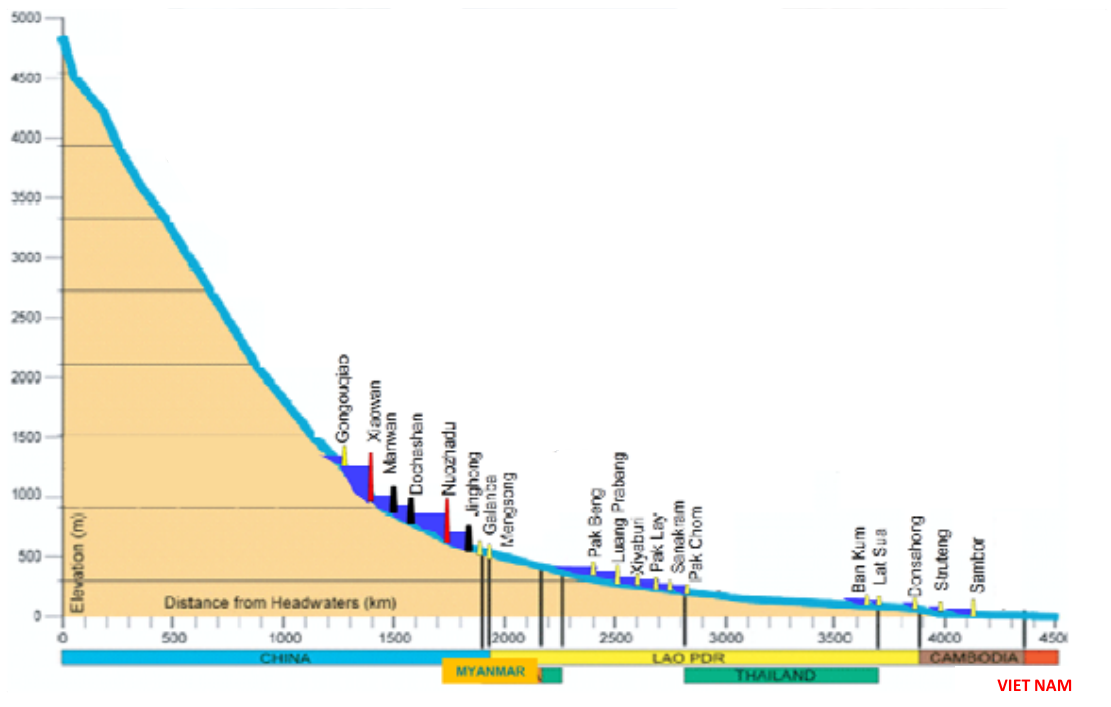
\includegraphics[scale=0.55]{mekong/11_proposed.png}
\caption{Mekong mainstream hydropower projects \cite{mrc}}
\end{figure}

Many of the benefits can be seen upstream, while many of the downsides can be seen downstream. This can lead to tensions between countries, as there is effectively a trade of wealth.\\

Lao PDR gains for example most from the overall power benefits directly associated with mainstream hydro power. Mainstream hydro power is less significant for the power sectors of Thailand and Vietnam, where the impact of the electricity prices are minor (less than 1.5\%).

Some downsides of the dams apply to different regions however. As a conservative estimate, the mainstream damming projects are expected to be responsible for one third of the reduction in nutrient and sediment loads of the Mekong River. This can translate into increasing food insecurity in the basin. If natural resources productivity is reduced, the countries most at risk are Cambodia and Lao PDR.

In March of 2010, the Mekong Delta reached its lowest water levels in 50 years. It opened the discussion between countries what effect hydropower dam development has on the Mekong Delta. \cite{globalissues} Looking back today, it seems that those discussions have not helped much. \\

The water levels reached its lowest point again in 2020. Dams are taking water out of the system during the wet season and putting it back in the dry season, resulting in the level of the river being too low for any sort of irrigation throughout the year. According to local farmers, the lower Mekong Delta is now salty for up to four months instead of the usual one month of the year, and entire fields of trees are are being killed by saltwater intrusion. \cite{voanews}



\begin{figure}[h]
\centering
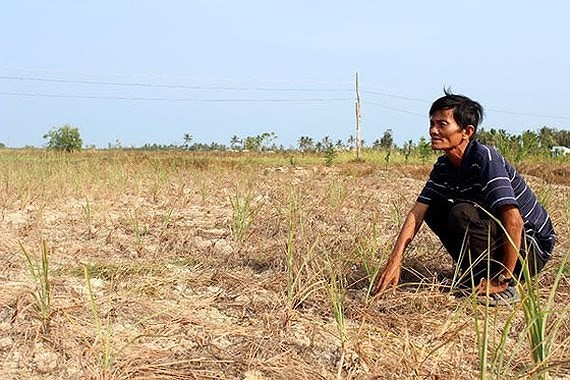
\includegraphics[scale=0.55]{mekong/41_paddy.jpg}
\caption{The drought-stricken Mekong River in Pak Chom district in the northeastern Thai province of Loei. 
\cite{voanews}}
\end{figure}

\subsubsection{Mitigation}
Several strategies have been developed for mitigating issues of the dams. Fish ladders may be a mitigation option for low dams on tributaries, but existing types and sizes of fish ladders cannot accommodate the intensity and diversity of fish migrations on the mainstream. Fishery reservoirs were proposed instead, but they would only be capable of producing 10\% of the lost capture fisheries.

If dams are continued to be used, the irrigation sector needs significant investment to re-equip it for use of reservoir water instead of using water from the Mekong Delta.
\newpage
\subsection{Subsidence}
Subsidence is a general term for downward vertical movement of the Earth's surface, which can be caused by both natural processes and human activities. 

Subsidence can be measured by 

From 2014-2019, Utrecht University launched a project called Rise and Fall that aims to enhance the capabilities of individuals and organisations to develop sustainable strategies for dealing with mainly groundwater extraction and land subsidence in the increasingly urbanising Mekong Delta. Throughout the years, they have generated several reports describing the issue of subsidence at hand. To describe the issue of subsidence in the Mekong Delta, it is best to take a look at this project's findings. \cite{riseandfall}

\subsubsection{Findings}

One of major findings of the project is that the elevation of the Mekong Delta is much lower than formerly estimated. By means of a high accuracy Digital Elevation Model generated using InSAR technology \cite{insar} it could be demonstrated that the average elevation of the delta is only 0,8 meter above mean sea level, instead of 2,6 meter as used as basic assumption by the international research community earlier. This means that the Mekong Delta is much more vulnerable to sea level rise as generally assumed. \cite{minderhoud2017}

The project researchers also showed that land subsidence takes place very fast. The Mekong Delta is subsiding at a rate of 1-5 centimetres a year, much higher than sea level rises following global warming. From a farmer’s perspective, this means that saline tidal water from the coast can enter the delta’s rivers much further inland and affect rice production.

\subsubsection{Cause}
The extraction of groundwater for drinking water, agriculture and fisheries in the Mekong Delta is the most probable cause of the dramatic land subsidence in this low-lying area. 

Researchers modelled the expected subsidence based on the amount of groundwater extraction and compared this expected subsidence for the actual subsidence. For the Mekong Delta, about 75\% of the cases of measured subsidence is at least matched by the best estimated modelled subsidence. \cite{minderhoud2017}

Land subsidence from ground water extraction occurs when large amounts of groundwater have been withdrawn from certain types of rocks, such as fine-grained sediments. The rock compacts because the water is partly responsible for holding the ground up. When the water is withdrawn, the rocks falls in on itself.

\subsubsection{Mitigation}
The top-down way groundwater governance is organised in Vietnam makes it difficult to define and implement local interventions. Still, designating specific areas for sedimentation is a suggested strategy to encourage elevation-building with nature in deltas. \cite{minderhoud2020}

One could also look into other ways to extract water, such as surface water treatment. While these actions won't solve subsidence, it delays future relative sea-level rise, giving the Mekong Delta time to adapt.
\newpage
\subsection{Salinization}
Salinization is the increase of salt concentration in soil and is, in most cases, caused by dissolved salts in the water supply. This supply of water can be caused by flooding of the land by seawater, seepage of seawater or brackish groundwater through the soil from below.

In April of 2016, a report has been made on the drought and salinity intrusion in the Mekong River Delta of Vietnam. It concluded that the salinity intrusion has worsened due to climate change and drought. It is useful to take a closer look at this report. \cite{salinity}

\subsubsection{The cause of salinity}
Salinity intrusion in the Mekong Delta is heavily caused by low water discharge from upstream of the Mekong River. Lesser rain falls in the Mekong basin lead to a reduction in upstream water flow to push back seawater. The situation worsens when there is drought and high temperatures in the region.

An oscillating warming and cooling pattern, referred to as the ENSO cycle, directly affects rainfall distribution in the Mekong Delta. El Niño and La Niña are the extreme phases of the ENSO cycle.

Recently, local authorities and farmers alike underestimated the drought and salinity intrusion conditions, thus rendered them unprepared for the impacts on aquaculture and agricultural production. Rice production, a main agricultural activity, was reduced in affected areas due to salinity intrusion, lack of freshwater and drought. 

\begin{figure}[h]
\centering
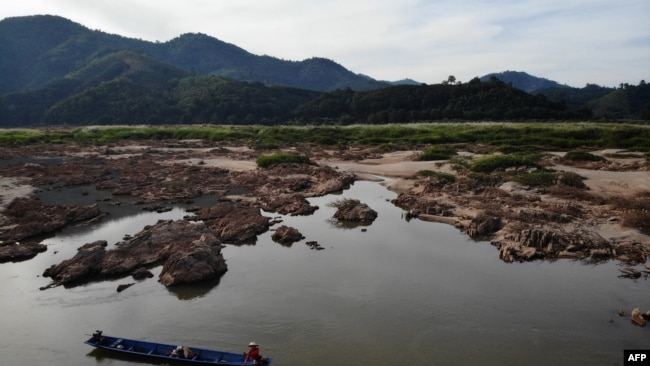
\includegraphics[scale=0.45]{mekong/12_drought.jpg}
\caption{A paddy field is hit by salinity in Mekong Delta 
\cite{saigononline}}
\end{figure}

These issues were largely caused by the below average rainfall in the Mekong basin due to the El Niño, as well as the use of hydropower dams. With insufficient upstream water flow to push back seawater, salinity intrusion increased in concentration and duration. This affected largely small-scale farmers and producers who have lower financial and technical capabilities to adapt to climate changes.

\subsubsection{Mitigation}

The Mekong Delta is heavily dependent on other countries and the climate for the flow of the Mekong River. Because of these uncontrollable dependencies, the Vietnam government opted for diversification. Shrimp farming was established along the coast, while farmers further inland started combining rice farming with freshwater aquaculture, mostly farming tilapia. Thanks to this development, Vietnam has grown into a significant exporter of shrimps and tilapia. \cite{wyrdykes}

\newpage
\subsection{Conclusion}
While there are many anecdotal reports available about the water availability and quality in the Mekong River, there exist relatively little data to validate these claims. Understanding what is happening to the Mekong River is a first step towards understanding what steps are necessary to mitigate problems. Such a step can only be achieved when there is sufficient monitoring, particularly monitoring over time.\\

\begin{figure}[h]
\centering
\includegraphics[scale=0.06]{mekong/02_dam.jpg}
\caption{Xiaowan Dam, Lancang (upper Mekong) River, China \cite{critnature}}
\end{figure}

Dams seem to cause a disturbance in the natural flow of the Mekong River, making both droughts and floods more common in the Mekong Delta. No constant stream of water upstream causes more saltwater intrusion downstream, making the agricultural industry less productive. Groundwater extraction causes subsidence, which in turn has very real consequences for the landscape of the delta.\\

\begin{figure}[h]
\centering
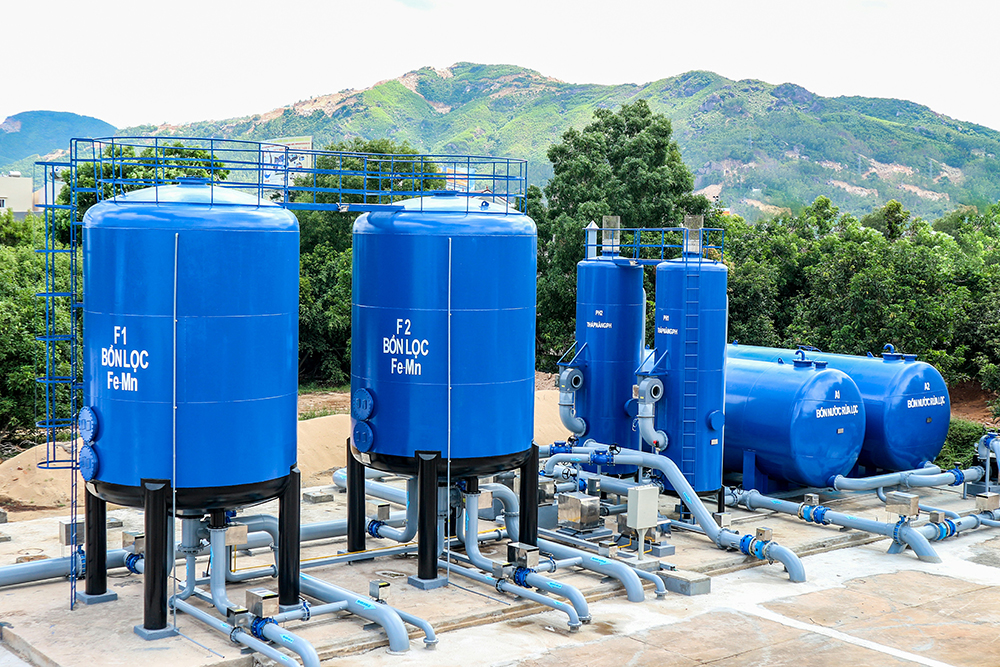
\includegraphics[scale=1]{mekong/01_groundwater.jpg}
\caption{Ground water treatment installation in Vietnam \cite{pernam}}
\end{figure}

As seen, the Mekong Delta's various sectors are facing numerous challenges, namely subsidence, salinization, and drought. These can be monitored by measuring variables such as conductivity, turbidity, and temperature continuously, across the Mekong River.

